\kapitola{Metodika}
Na začátku je potřeba provést analýzu problému s ohledem na požadavky stanovené konzultacemi s vedoucím. Návrh bude také zahrnovat experimenty, které budou s neuroevolucí provedeny.

Po návrhu bude následovat implementace daného řešení. Popis řešení bude přidán do této práce. V průběhu implementace bude také kód a návrh postupně upravován na základě požadavků, které se mohou objevit až při implementaci navrženého řešení.

Po implementaci bude následovat realizace a vyhodnocení experimentů popsaných v návrhu.

Na závěr proběhne vyhodnocení řešení s návrhem možných zlepšení.
\kapitola{Analýza problému}
Tato kapitola se zabývá analýzou funkčních a nefunkčních požadavků pro softwarové řešení. Požadavky vznikaly na základě konzultace s vedoucím a vlastní invencí.

\sekce{Funkční požadavky}
Funkční požadavky jsou rozděleny do několika kategorii.

\podsekce{Simulace}
Vyhodnocování agenta bude probíhat jeho nasazením v simulovaném prostředí. Fitness bude pak vyhodnocena na základě jeho akcí v prostředí.
\begin{itemize}
	\item Testovací prostředí musí být pro všechny agenty stejné
	\item Fitness funkce musí být deterministická
	\item Fitness by měla být zjistitelná kdykoliv v průběhu simulace
	\item Simulace by měla být konfigurovatelná 
	\item Možnost změny obtížnosti simulace pro agenta
	\item Měla by existovat možnost spuštění více instancí simulace v rámci jednoho programu
\end{itemize}
\podsekce{Vizualizace}
Průběh algoritmu je třeba zobrazit.
\begin{itemize}
	\item Je třeba provést grafickou vizualizaci fyzikální simulace
	\item Při zobrazení by mělo být možné vyčíst stav agenta (fitness, senzory, ...) 
	\item Možnost vizualizace průběhu simulace v reálném čase (například pro její demonstraci v předmětu VUI2)
\end{itemize}

\podsekce{Experimenty}
Práce zahrnuje vyhodnocování agenta v různých podmínkách z tohoto vychází následující požadavky:

\begin{itemize}
\end{itemize}

\sekce{Nefunkční požadavky} 
Spolu s funkčními požadavky jsou na řešení kladeny také požadavky nefunkční.
\begin{itemize}
	% TODO: Předělat do formátu Něco - ....
	\item Škálovatelnost - Možnost spustit a vykreslit libovolné množství simulací
	\item Rychlost simulace. - Simulace by měla být schopná samostatně běžet alespoň rychlostí 30 snímků za vteřinu.
	\item Robustnost - Simulace by měla být odolná neočekávaným situacím
	\item Portabilita - bylo třeba zajistit, aby šlo kód rozběhnout v různých platformách v různých konfigurací.
	\item Robustnost - Simulace by si měla poradit s neočekávanými vstupy, jako je třeba \textbf{NaN}, který vychází z neuronové sítě.
\end{itemize}

\kapitola{Návrh řešení}


\kapitola{Implementace}
Vlastní práce se skládá ze dvou částí klientská část, která slouží k~vizualizaci algoritmu a zobrazení výsledků ze serverové části. Serverová část pro maximální urychlení simulace. 

\sekce{Simulace}
Simulace je realizovaná jako knihovna pro Node.js, lze jí tedy použít jak u klientské částí, tak u serverové části. Poskytuje kompletní fyzikální simulaci agenta, prostředí ve kterém se pohybuje, jeho ovládání a výpočet fitness funkce. Součástí simulačního prostředí je také kód pro její vizualizaci.


Rychlost byla zajištěna implementací profilovacího programu (\textbf{benchmark.js} ve složce simulation), který spouští simulaci na předem připravené populaci jedinců. Výstupem je pak doba, za jakou jí vyhodnotil na jednom jádře procesoru. Tento údaj byl pak používán při implementaci simulace pro orientační představu, jak moc případné změny v kódu ovlivňují rychlost samotné simulace. Dále byla simulace podrobena občasnému profilování v klientské částí s pomocí vývojářských nástrojů prohlížeče chrome, na kterém simulace jede nejlépe.

Nenáročnost, která souvisí s rychlostí pak byla zajištěna tím, že bylo v průběhu psaní kódu dbáno na to, aby v průběhu simulace nedocházelo k přebytečným alokacím, které by nejen že mohli způsobit přebytečný nárůst požadované paměti ale způsobovali by také nepředvídatelné zpomalení, které s sebou přináší jazyk využívající garbage kolektor.

Robustnost je podrobněji vysvětlená v sekci \ref{sec:fitness} a popis toho, jak bylo dosaženo stejných podmínek pro všechny agenty lze nalézt v návrhu \ref{sec:ECS} především v popisu RoadManageru.

\sekce{Serverová část}
Serverová část vyhodnocuje jednotlivé jedince distribuovaně s~pomocí fronty úkolů. Frontu poskytuje knihovna \textbf{Bull}, která používá \textbf{Redis} pro správu údajů o~jednotlivých úkolech.

Cílem byl návrh robustního systému, který v~ideálním případě rozloží výpočetní zátěž mezi jednotlivé uzly rovnoměrně. Dalším požadavkem byla možnost odpojení kdykoliv kteréhokoliv z počítačů, jelikož ne všechny bylo možné nechat běžet přes noc.

\sekce{Výpočetní cluster}
\label{sec:cluster}
Ukázalo se, že vyhodnocování simulace zabírá neúměrné množství času a to i na nejvýkonnějším dostupném počítači. 
Například vyhodnocení jedné generace populace o~1024 jedincích zabralo ~290 s~na nejsilnějším dostupném pc. Z~tohoto důvodu bylo rozhodnuto o~distribuce výpočetní zátěže mezi více počítačů. Byl vytvořen výpočetní cluster se specifikací popsanou v~tabulce \ref{table:hw_table}.
\begin{table}[h!]
	\centering
	\begin{tabular}{|l|c|c|c|}
		\hline 
		Procesor & RAM & Počet & Architektura\\ 
		\hline 
		S5P6818 Octa core & 1 GB & 2 & arm64 \\ 
		\hline 
		Broadcom BCM2837B0 quad-core & 1 GB & 1 & arm32 \\ 
		\hline 
		Phenom X4 965 & 8 GB & 1 & x64 \\ 
		\hline
		Intel Core i5-2300 & 4 GB & 1 & x64 \\ 
		\hline 
		Intel atom x5-Z8350 & 2 GB & 1 & x64 \\ 
		\hline
		Cortex-A5 & 1 GB & 1 & armv7l \\
		\hline
	\end{tabular} 
	\caption{Použitý hardware}
	\label{table:hw_table}
	
\end{table}
\podsekce{Vyhodnocování rychlosti}
Lze i namítnout, že se zde projevuje určitá režie při síťové komunikaci se serverem, což může být zdrojem určitého zpomalení.

Pro ověření rychlosti bylo provedeno měření výkonu clusteru a jeho porovnání s nejvýkonnější dostupnou sestavou. Měření bylo provedeno nad náhodně vygenerovanými populacemi. Jelikož se simulace může ukončit předčasně (například při kolizi s překážkou) byla simulace provedena pro každou velikost $10\times$ a výsledek byl zprůměrován. Naměřená data lze nalézt v tabulce \ref{table:clusterBenchmark} ze které vychází obrázek \ref{fig:benchmarkcluster} na kterém lze vidět výsledky tohoto srovnání. 

Porovnání rychlosti clusteru s nejvýkonnějším dostupným počítačem ukazuje, že cluster je ve většině případů skoro stejně nebo  výrazně rychlejší než samostatný výpočet. Jediné dvě naměřené instance, kde to neplatí je u populací o velikosti 100 a 200, kde si cluster vede mírně hůře, než nejvýkonnější dostupná sestava. Toto lze vysvětlit, jak přítomností méně výkonného hardwaru v clusteru (především se jedná o S5P6818) na které se musí u menších populací čekat. Dalším vysvětlením mohou být výše uvedené důvody.

Je nutné však podotknout, že proměnlivá doba u vyhodnocování jedince znamená, že měření není zcela přesné. Nicméně lze na základě dat usoudit, že u větších populací dochází k přibližně $2\times$ zrychlení.

\begin{figure}[H]
	\centering
	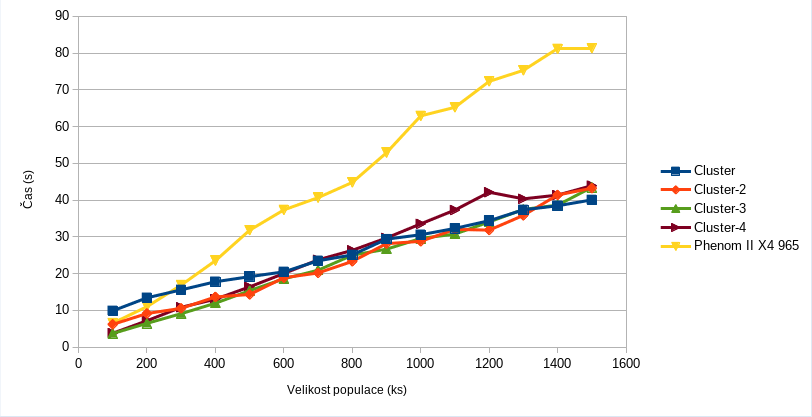
\includegraphics[scale=0.7]{benchmarkCluster}
	\caption{Porovnání rychlosti clusteru s jedním PC}
	\label{fig:benchmarkcluster}
\end{figure}

\begin{table}[H]
	\centering
	\begin{tabular}{|l|c|c|}
		\hline
		Počet & Cluster & Phenom II X4 965 \\
		\hline
		100     & 9.6277  & 6.5186           \\
		\hline
		200     & 13.2919 & 10.9839          \\
		\hline
		300     & 16.5404 & 16.8723          \\
		\hline
		400     & 17.9967 & 23.5019          \\
		\hline
		500     & 20.3733 & 31.7831          \\
		\hline
		600     & 22.4781 & 37.3242          \\
		\hline
		700     & 25.1767 & 40.66            \\
		\hline
		800     & 27.5549 & 44.8019          \\
		\hline
		900     & 30.7077 & 52.8829          \\
		\hline
		1000    & 32.8463 & 62.8967          \\
		\hline
		1100    & 33.3567 & 65.2363          \\
		\hline
		1200    & 36.0618 & 72.2926          \\
		\hline
		1300    & 39.4703 & 75.2937          \\
		\hline
		1400    & 42.4464 & 81.1193          \\
		\hline
		1500    & 44.9014 & 81.3101          \\
		\hline
	\end{tabular}
	\caption{Naměřená data}
	\label{table:clusterBenchmark}
\end{table}

\podsekce{Docker swarm}
Pro snadnou distribuci a správu byly všechny počítače zorganizovány do docker swarmu. Docker swarm obsahoval jednoho manažera (Broadcom BCM2837B0 quad-core), který zároveň spouštěl klientskou aplikaci a další služby:

\begin{enumerate}
	\item \textbf{Portainer} pro správu clusteru
	\item \textbf{Arena} webové UI pro správu knihovny \textbf{Bull}
	\item \textbf{Redis} používaný knihovnou \textbf{Bull}
\end{enumerate}

Na manažerovy nebyl spuštěn zpracovatel, aby se zabránilo jeho přetížení (manažer swarmu by měl být vždy dostupný).

Použití docker swarmu umožňuje především snadné nasazení a správu zpracovávajících procesů. Zároveň zajišťuje, že všechny instance zpracovatelů mají unifikovanou konfiguraci, což je zvláště důležité pro dosažení konzistentních výsledků.

\begin{figure}[H]
	\centering
	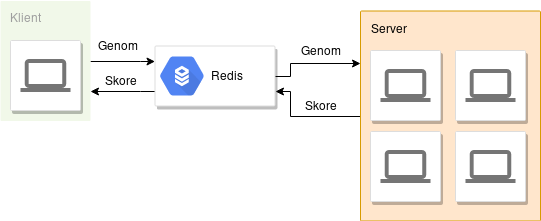
\includegraphics[scale=0.5]{distributed}
	\caption[Schéma distribuovaných výpočtů]{Schéma distribuovaných výpočtů}
	\label{fig:distributed}
\end{figure}

Tento přístup má několik výhod a to:

\begin{enumerate}
	\item Robustnost - Pokud jeden nebo více zpracovatelů selže (je například odpojen ze sítě) je možné pokračovat ve vyhodnocování (neúspěšný úkol lze vrátit zpátky do fronty). Toto v kombinaci s výše zmíněným docker swarmem znamená, že jakýkoliv výpočetní uzel lze kdykoliv vypnout a po znovu zapojení do sítě si načte nejnovější konfiguraci a začne znovu vyhodnocovat bez potřeby jakékoliv manipulace s jakoukoliv částí swarmu.
	\item Dobré rozložení zátěže - Jelikož si zpracovatel vytahuje úkoly z~fronty, je vždy optimálně zatížen, a není třeba řešit rozložení mezi různě výkonnými a zatíženými počítači.
	\item Škálovatelnost - problém lze škálovat až do doby, kdy počet procesorů nepřesáhne počet potřebných simulací. Chceme-li tedy vypočítat generaci o tisíci jedincích můžeme na ně nasadit až tisíc procesorů.
\end{enumerate}

\podsekce{Monitorování stavu}
Pro monitorování stavu algoritmu byla použita webová aplikace Grafana. Jak jíž bylo řečeno v sekci \ref{sec:grafana} jedná se o nástroj pro snadnou vizualizaci dat v databázi. V případě této práce posloužila k vytvoření jednoduchého kontrolního panelu, který obsahoval následující informace:
\begin{itemize}
	\item Graf zobrazující fitness nejlepšího/nejhoršího jedince dle generací
	\item Textové pole, které obsahuje nejlepší genom
	\item Numerické pole, které obsahuje počet generací
	\item Graf zobrazující dobu výpočtu dle generací
\end{itemize}
\begin{figure}[H]
	\centering
	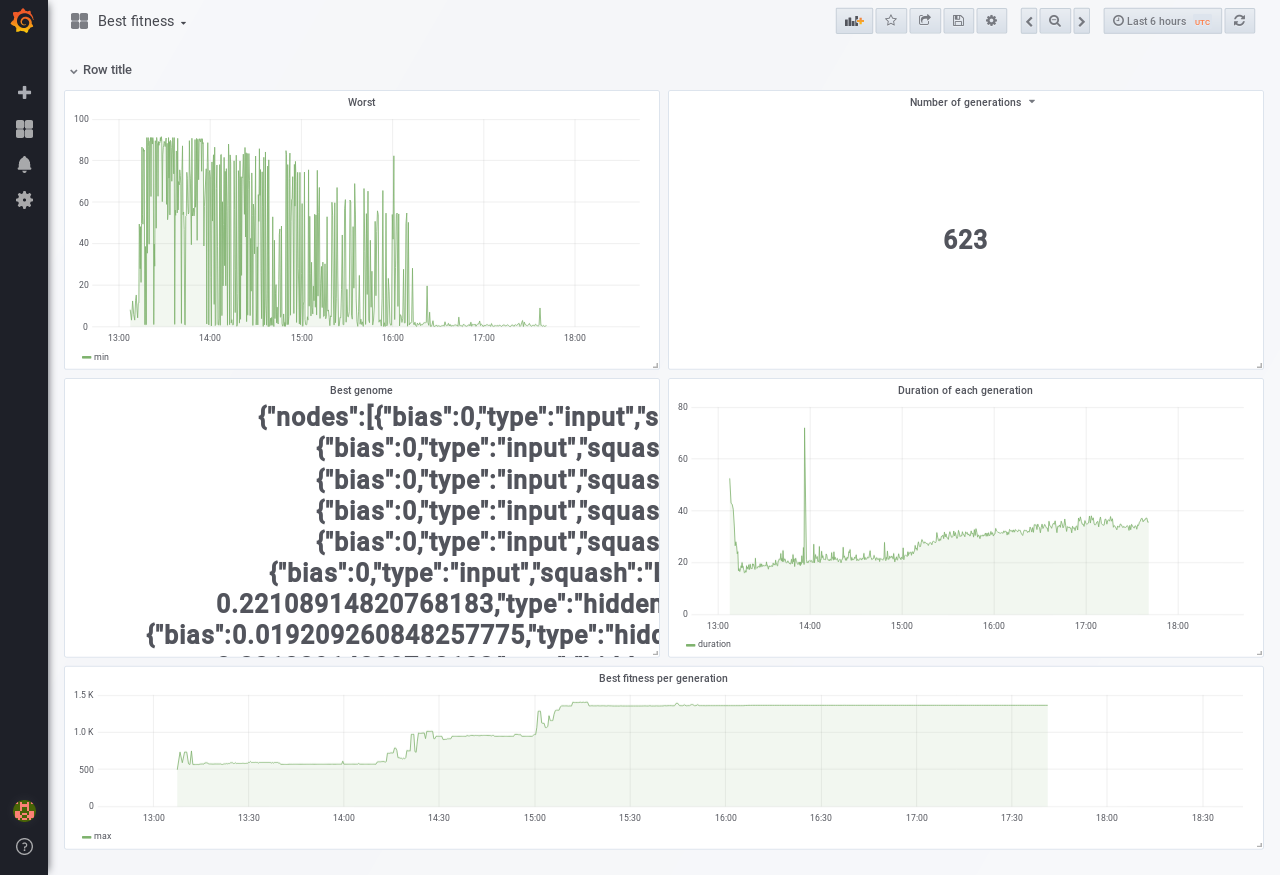
\includegraphics[width=0.7\linewidth]{grafana}
	\caption{Kontrolní panel v aplikaci grafana}
	\label{fig:grafana}
\end{figure}

\kapitola{Klientská část}
Klientská část byla navržena tak, aby byla schopná vizualizovat průběh algoritmu NEAT a zároveň měla možnost znovu vyhodnocení existujících genomů vygenerovaných serverovou částí. První požadavek vznikl na základě konzultace s vedoucím, který chtěl algoritmus NEAT demonstrovat v hodinách předmětu VUI2. Druhý požadavek vznikl z důvodu potřeby vizualizace řešení, které generoval sever.

\sekce{Vizualizace}
Vizualizace se skládá z jednoduchého rozhraní, které lze vidět na obrázku \ref{fig:visualization}. V horní části je graf, zobrazující průběh genetického algoritmu. Lze v něm nalézt fitness nejlepšího, nejhoršího a průměrného jedince v populaci.

Další část se skládá z konfigurovatelného množství simulačních prostředí. Jednotliví jedinci v generaci jsou pak rovnoměrně rozloženi mezi všechna simulační prostředí a uživatel může pozorovat vývoj jedinců v reálném čase.

Poslední tlačítko slouží k urychlení simulace. Způsobí to, že se simulace začne obnovovat bez vykreslování. Toto jí značně zrychlí.

\begin{figure}[h!]
	\centering
	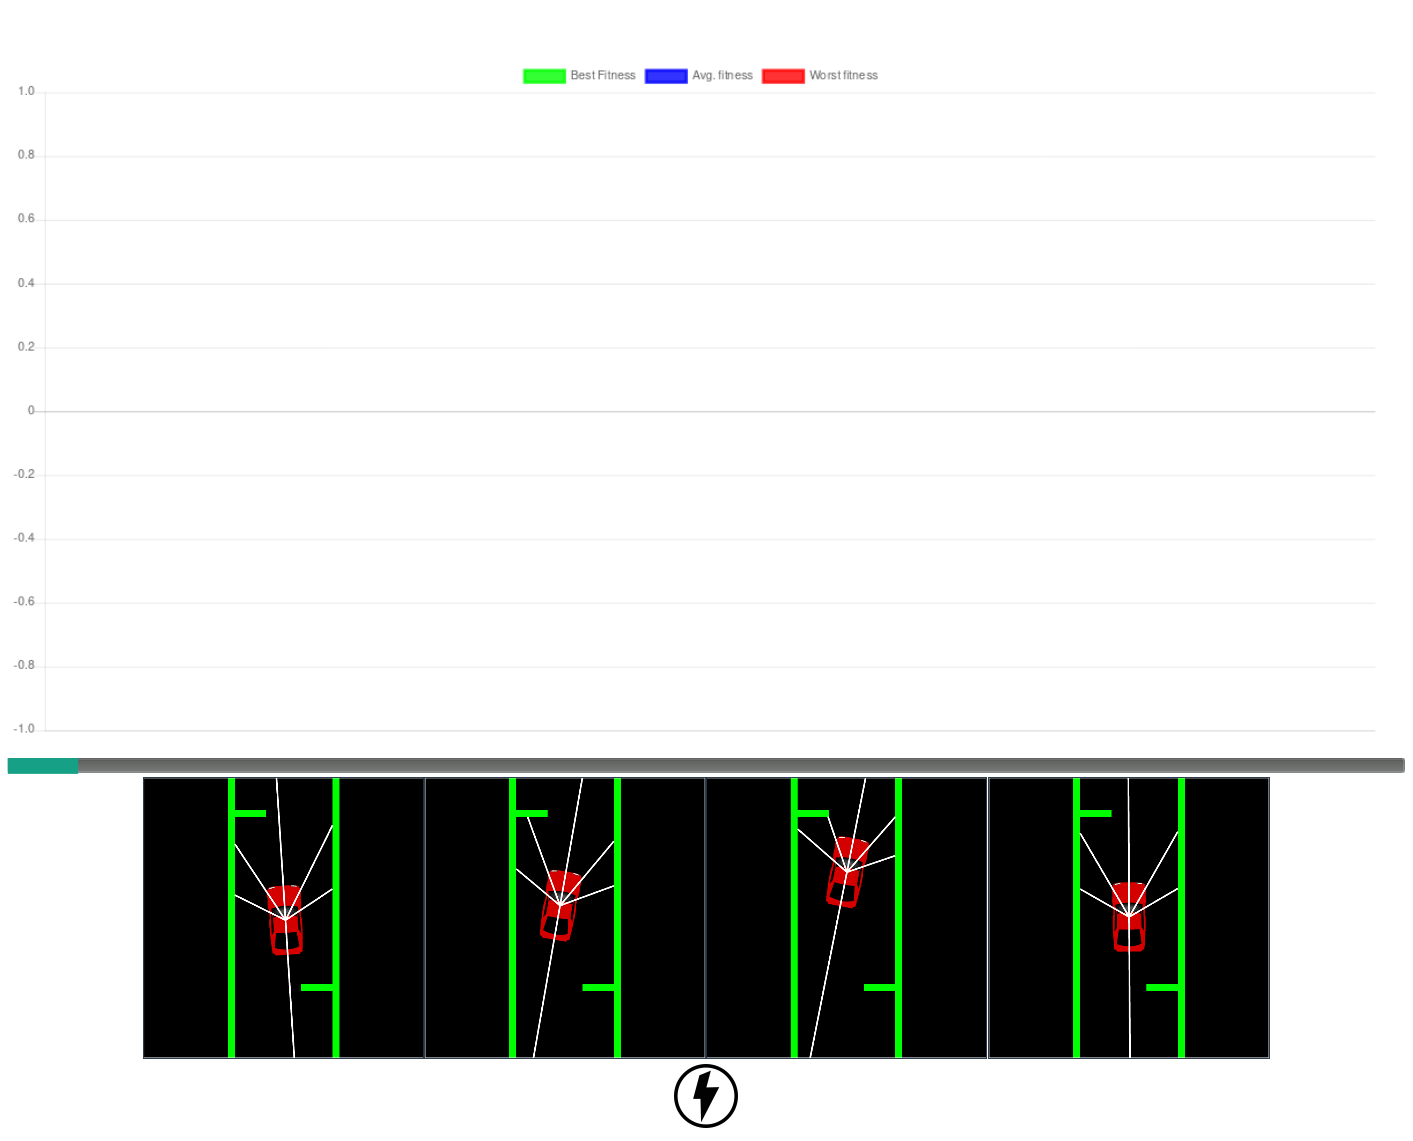
\includegraphics[width=0.6\linewidth]{visualization}
	\caption{Uživatelské rozhraní klientské části}
	\label{fig:visualization}
\end{figure}


\kapitola{Experimenty}
Po návrhu simulačního prostředí byl agent vyzkoušen v~několika situacích se stupňující se obtížností. Každá simulace probíhala s~1000 jedinci po 2000 generací. Ačkoliv je pravděpodobné, že by delší doba evaluace by pravděpodobně vyústila v lepší výsledky její výpočet v různých konfiguracích se ukázal jako příliš časově náročný navíc empirické pozorování ukázalo, že tato konfigurace poskytuje dostatečně dobré výsledky za snesitelný čas. 

S ohledem na časovou náročnost výpočtů (výpočet tisíce generací trvá na výpočetním clusteru přibližně 5 hodin) byly zkoumany jen tyto konfigurace:
\sekce{Nekonečná silnice ve tvaru I}
Agent byl umístěn do nekonečné rovné silnice ve tvaru I. Cílem bylo pozorovat, zda se agent bude schopný naučit řídit rovně. Agent po tisící generací dosáhl fitness 3 500 a naučil úspěšně kývavým pohybem udržet uprostřed vozovky.
\begin{figure}[h]
	\centering
	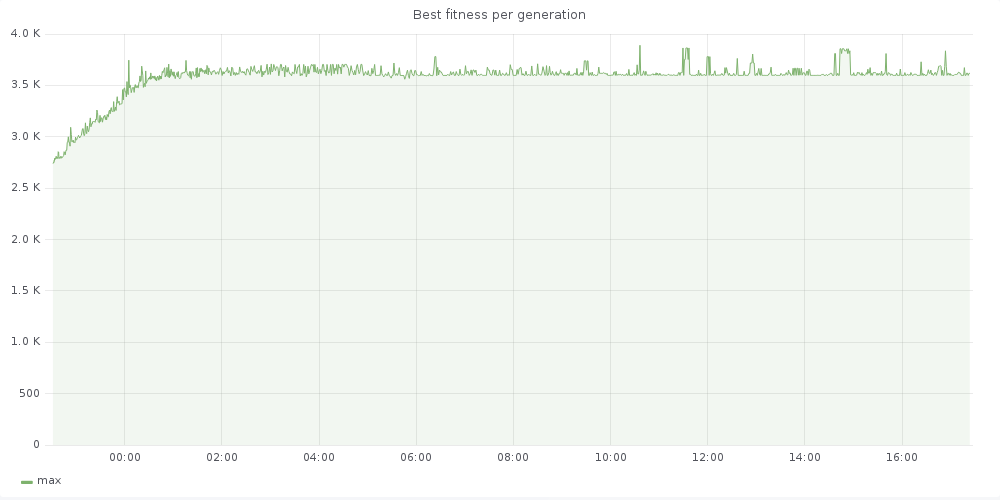
\includegraphics[scale=0.4]{I_fitness}
	\caption{Fitness agenta v průběhu času}
	\label{fig:i-experiment}
\end{figure}

\kapitola{Možná vylepšení}
Tato kapitola se bude zabývat možnými vylepšení současného řešení.

\kapitola{Závěr} 